\section{Evaluation}

We evaluate \system{}'s ability to avoid a given country, its performance,
and its storage and measurement costs.

\subsection{Country Avoidance}

We measured \system{}'s effectiveness in achieving country avoidance.  We did so by first 
calculating the number of {\it default} paths that avoid a given country.  Then 
we added a single relay, and calculated how many domains the client could 
access without traversing through the given country.  We repeated this approach for 
the remaining relays.  We conducted the evaluation under the condition that 
the client wished to avoid different countries when accessing the Netherlands top 
100 domains; Figure~\ref{fig:avoidance_eval} shows these results.  Each 
line represents the fraction of domains accessible while avoiding the country that 
the line represents.  For example, 46\% of domains are accessible without traversing 
the U.S. when \system{} is not being used (zero relays), and if \system{} is 
used, then 63\% of domains are accessible without traversing the U.S.

\begin{figure}[t!]
\tiny
\centering
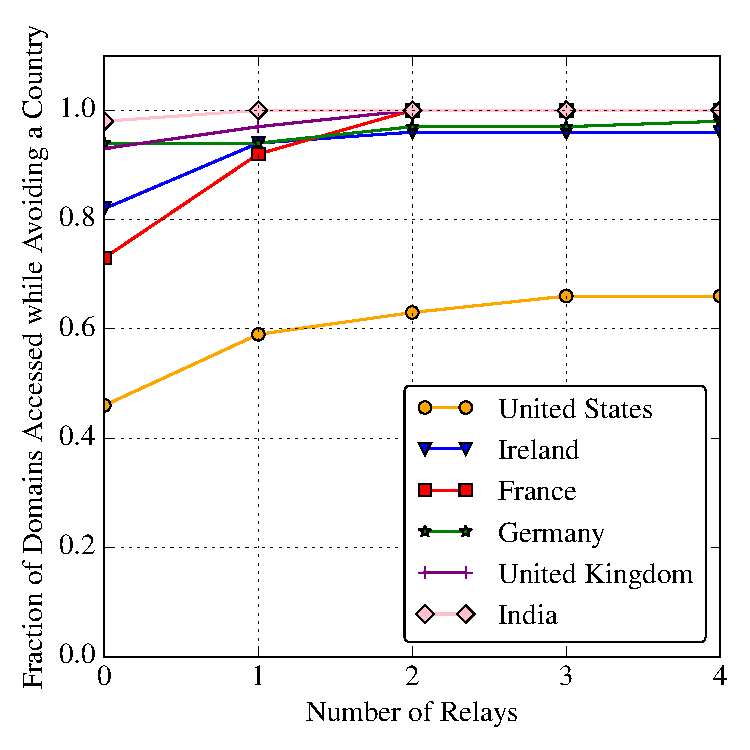
\includegraphics[width=.5\textwidth,height=6cm]{avoidance_n_relays}
\caption{The effect of the number of relays on avoidance, for a client
  in the Netherlands. We tested \system{} with up to nine relays.}
\label{fig:avoidance_eval}
\end{figure}

It is evident that \system{} helps a client avoid a foreign country,
as the fraction of domains accessible without traversing the specified
country without \system{} is lower than with \system{}.  Additionally,
adding the first relay provides the greatest benefit, while subsequent
relays offer diminishing returns.  Figure~\ref{fig:avoidance_eval}
clearly shows that avoiding the U.S. is much more difficult (or
impossible) than any other country.  Only 63\% of domains can be
accessed while avoiding the U.S., whereas almost all domains can be
accessed while avoiding any other given country.
%This confirms the results presented in Section \ref{avoid_results}, and 
%emphasizes how crucial the systematization of the measurements is for enabling 
%\system{}.

It is important to note that \system{} cannot guarantee that a country is 
avoided because for some domains, the path must go through the unfavorable 
country, as evidenced by our results for avoiding the United States.  Despite 
this lack of guarantees, the system reduces the number of requests that 
transit the unfavorable country; additionally, the client can learn which domains 
are not accessible without passing through the unfavorable country, and can then 
decide whether or not they want to fetch that page.  

\subsection{Performance}
To measure the performance of \system{}, we measure both 
the throughput and latency.

To measure throughput, we ran {\tt wget} for each 
of the top 100 domains from the client machine in the Netherlands 
using an oracle-generated PAC file.  Because different relays could have been 
used to avoid a single domain, the oracle selected a random relay from those 
that would allow the client to avoid the country.  The oracle generated 
ten PAC files for a client in the Netherlands who wishes to avoid the United States,
 randomly selecting a relay for domains that could have used 
different relays, and {\tt wget} was used for the top 100 domains for each 
PAC file generated.  Based on the {\tt wget} output, we calculate the number 
of seconds to access content using our system and take the average across the 
ten experiments. 

\begin{figure}[t]
\centering
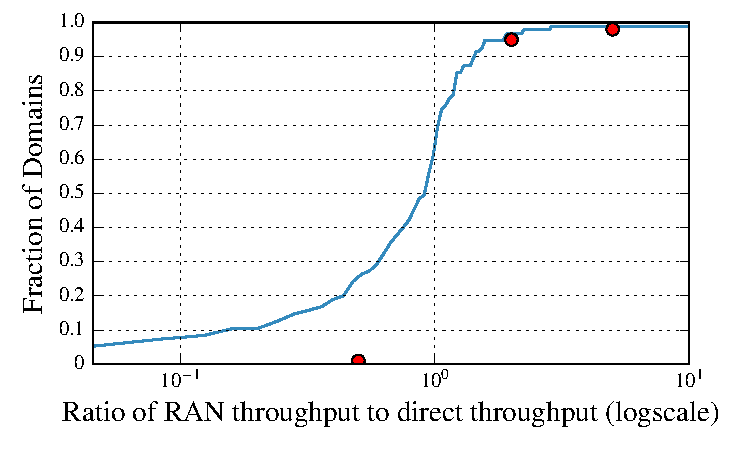
\includegraphics[width=.5\textwidth]{throughput}
\caption{The ratio of RAN throughput to direct throughput.  
The points on the graph are taken from the RON study and represent a ``normal'' overlay network's 
performance.} 
\label{fig:throughput}
\end{figure}

Figure \ref{fig:throughput} shows a CDF of the ratio of \system{}
throughput to direct throughput.  The throughput of
\system{} is not significantly worse than that of default paths.  
In some cases the performance of \system{} is {\it better} than
that of default paths.  Such improvements could be a result of the
relays keeping local traffic local, or due to a closer content replica
being selected.  These results show that \system{}'s performance is
comparable to the performance of accessing domains without \system{}.
Figure \ref{fig:throughput} also compares \system{}'s throughput to
RON's throughput, illustrated with the red dots.  \system{} performs
worse than RON ($x < 1$), which is expected, as the detours that
\system{} introduces inherently inflates paths.  Interestingly, both
RON and \system{} improve throughput for a similar fraction of samples
($x>1$).

To measure the latency of \system{}, we ran {\tt curl} to each of the 
top 100 domains from the client in the Netherlands, while using the ten
oracle-generated PAC files. This provided the time to first byte (TTFB); we 
found the average TTFB when accessing content using \system{} and 
found the TTFB when using direct paths; the results are shown in Figure \ref{fig:latency}.  
The median TTFB for direct paths is 68.5~ms; for \system{} paths the
median is 100.8~ms; 90th percentile TTFB is 22.5~ms and 40.4~ms, respectively.  


\begin{figure}[t]
\centering
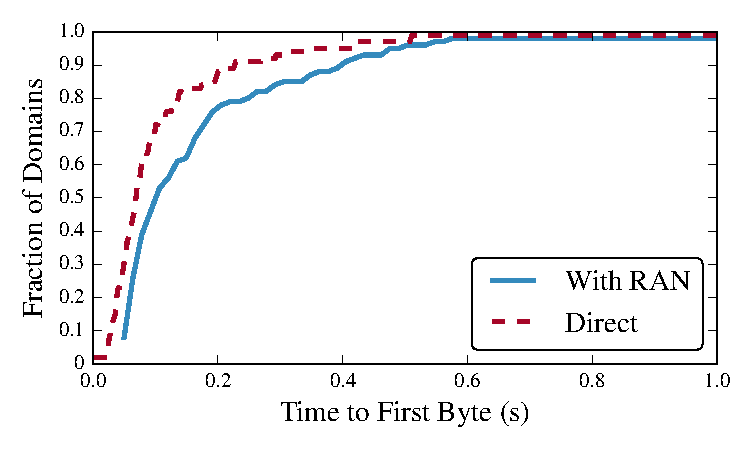
\includegraphics[width=.5\textwidth]{latency}
\caption{Time to First Byte for \system{} and direct paths.}
\label{fig:latency}
\end{figure}


\subsection{Storage and Measurement Costs}

As the number of clients increase, and subsequently the number of paths being 
computed increases, the amount of storage must remain reasonable.  The storage 
used by paths can be calculated as
$DR + 2CR + CD$
where $D$ is the number of domains; $R$ is the number of relays; and $C$ is the
number of ASes from which \system{} measures.
The storage required for a single client, 100 domains, and nine relays is
480~KB.  Because there is a single PAC file for all clients in 
a country, $C$ will grow much slower than if there was a different PAC file for 
each individual client.  There are 196 countries; if \system{} computed
paths and a PAC file for each country, with 100 domains, and 
three relays required storage would be only 94~MB, making it
feasible to increase the number of relays and domains.

RIPE Atlas credits are also a limited resource.  Cost is proportional to
$C \cdot (R+D)$.
Each traceroute costs 60 RIPE Atlas credits, so one set of measurements
for one client, 100 domains, and nine relays costs 6,180 
credits; because these paths are updated each hour, then 
the daily credit cost is 148,320 credits.  In return for hosting a RIPE Atlas 
probe, we earn 216,000 credits per day, which will support our existing 
prototype.  In order to provide for more clients, more domains, or more 
resources, we can tune the system to re-compute paths less frequently,
as we discuss in Section~\ref{sec:discussion}.
